\newpage{\clearpage}
\chapter{Resultados del proyecto}

\section{Primer Prueba}

Se procedió a realizar la primer prueba con nuestro medidor y debido que en ese momento el mundo se encontrabá en la pandemia del COVID-19, tocó realizar pruebas con cargas domésticas las culaes fueron las siguientes:
\begin{itemize}
    \itemsep0em
    \item Bombillo de 9 W.
    \item Portatil dell.
    \item Osciloscopio.
    \item Raspberry.
    \item TV de 111 W.
    \item Play Station 3,
    \item Parlantes.
    \item Licuadora.
    \item Licuadora Nutribullet.
    \item Plancha de 1000 W.
\end{itemize}
\begin{table}[htbp]
    \centering
    \caption{Resultados de la prueba Nº 1}
      \begin{tabular}{|l|r|r|r|}
      \toprule
      \multicolumn{1}{|c|}{\multirow{2}[4]{*}{CARGA}} & \multicolumn{1}{c|}{MULTÍMETRO} & \multicolumn{2}{c|}{TARJETA} \\
  \cmidrule{2-4}          & \multicolumn{1}{l|}{Corriente} & \multicolumn{1}{l|}{Voltaje} & \multicolumn{1}{l|}{Corriente} \\
      \midrule
      Bombillo led de 9WT & 0,0772 & 122   & 0,84175682 \\
      \midrule
      Portatil, osciloscopio, Raspberry, TV(111W), Play 3, Parlantes & 1,4   & 122   & 2,48453856 \\
      \midrule
      Licuadora & 2,11  & 122   & 3,10783076 \\
      \midrule
      Licuadora pequeña & 1,46  & 122   & 2,32913756 \\
      \midrule
      Licuadora + licuadora pequeña & 3,87  & 121   & 5,06727028 \\
      \midrule
      Plancha de 1000W & 9,2   & 118   & 10,7248316 \\
      \midrule
      Licuadora + licuadora pequeña + plancha & 12,55 & 116   & 14,6785336 \\
      \bottomrule
      \end{tabular}%
    \label{tab:resultado1-1}%
  \end{table}%
  

  \begin{table}[htbp]
    \centering
      \begin{tabular}{|c|c|r|r|r|r|}
      \toprule
      \multicolumn{2}{|c|}{OSCILOSCOPIO} & \multicolumn{2}{c|}{\cellcolor[rgb]{ .557,  .663,  .859}Diferencias de corriente (A)} & \multicolumn{2}{c|}{\cellcolor[rgb]{ .557,  .663,  .859}Diferencia de voltaje(V)} \\
      \midrule
      \multicolumn{2}{|c|}{Voltaje} & \multicolumn{1}{c|}{\cellcolor[rgb]{ .557,  .663,  .859}Error Absoluto} & \multicolumn{1}{c|}{\cellcolor[rgb]{ .557,  .663,  .859}Error relativo} & \multicolumn{1}{c|}{\cellcolor[rgb]{ .557,  .663,  .859}Error Absoluto} & \multicolumn{1}{c|}{\cellcolor[rgb]{ .557,  .663,  .859}Error relativo} \\
      \midrule
      \multicolumn{2}{|c|}{119,93} & \cellcolor[rgb]{ .557,  .663,  .859}0,764556821 & \cellcolor[rgb]{ .557,  .663,  .859}990\% & \cellcolor[rgb]{ .557,  .663,  .859}2,07 & \cellcolor[rgb]{ .557,  .663,  .859}2\% \\
      \midrule
      \multicolumn{2}{|c|}{119,53} & \cellcolor[rgb]{ .557,  .663,  .859}1,084538555 & \cellcolor[rgb]{ .557,  .663,  .859}77\% & \cellcolor[rgb]{ .557,  .663,  .859}2,47 & \cellcolor[rgb]{ .557,  .663,  .859}2\% \\
      \midrule
      \multicolumn{2}{|c|}{119,63} & \cellcolor[rgb]{ .557,  .663,  .859}0,997830763 & \cellcolor[rgb]{ .557,  .663,  .859}47\% & \cellcolor[rgb]{ .557,  .663,  .859}2,37 & \cellcolor[rgb]{ .557,  .663,  .859}2\% \\
      \midrule
      \multicolumn{2}{|c|}{119,87} & \cellcolor[rgb]{ .557,  .663,  .859}0,869137564 & \cellcolor[rgb]{ .557,  .663,  .859}60\% & \cellcolor[rgb]{ .557,  .663,  .859}2,13 & \cellcolor[rgb]{ .557,  .663,  .859}2\% \\
      \midrule
      \multicolumn{2}{|c|}{118,56} & \cellcolor[rgb]{ .557,  .663,  .859}1,197270279 & \cellcolor[rgb]{ .557,  .663,  .859}31\% & \cellcolor[rgb]{ .557,  .663,  .859}2,44 & \cellcolor[rgb]{ .557,  .663,  .859}2\% \\
      \midrule
      \multicolumn{2}{|c|}{120} & \cellcolor[rgb]{ .557,  .663,  .859}1,524831581 & \cellcolor[rgb]{ .557,  .663,  .859}17\% & \cellcolor[rgb]{ .557,  .663,  .859}-2 & \cellcolor[rgb]{ .557,  .663,  .859}2\% \\
      \midrule
      \multicolumn{2}{|c|}{114,5} & \cellcolor[rgb]{ .557,  .663,  .859}2,128533554 & \cellcolor[rgb]{ .557,  .663,  .859}17\% & \cellcolor[rgb]{ .557,  .663,  .859}1,5 & \cellcolor[rgb]{ .557,  .663,  .859}1\% \\
      \midrule
      \multicolumn{2}{|c|}{**Promedio de diferencia =} & \cellcolor[rgb]{ .557,  .663,  .859}1,22381416 & \cellcolor[rgb]{ .557,  .663,  .859}177\% & \cellcolor[rgb]{ .557,  .663,  .859}1,568571429 & \cellcolor[rgb]{ .557,  .663,  .859}2\% \\
      \bottomrule
      \end{tabular}%
    \label{tab:resultado1-2}%
  \end{table}%

  **El valor de referencia es el osciloscopio o muiltimetro y el experimental es el valor de la tarjeta\\

  \begin{figure}[H]
    \begin{center}
        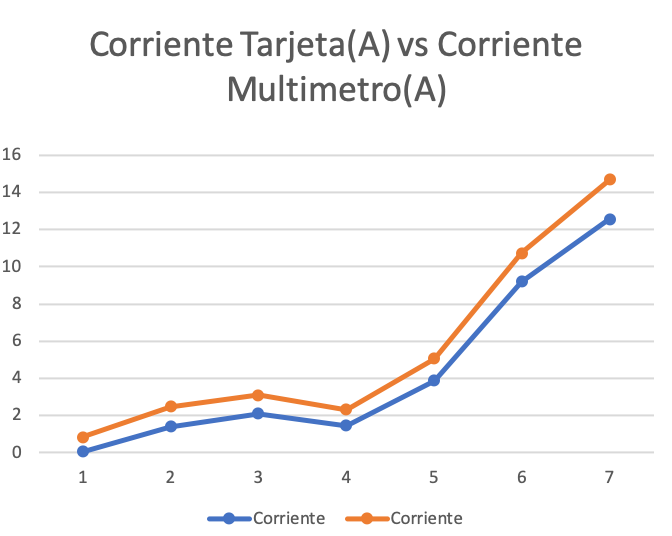
\includegraphics[width = 10cm]{4Resultados/prueba-1.png}
        \caption{ Corriente Tarjeta vs Corriente Multímetro } 
        \label{fig:prueba1}
   \end{center}
\end{figure}

En esta prueba, solo se comparó los registros de corriente rms y voltaje rms que entrega el software con un amperimetro y un osciloscopio midiendo voltaje.
 De igual manera, se calculó un error absoluto y relativo para después ajustar los datos.

 En la figura \ref{fig:prueba1}, la corriente de la tarjeta, tiene presición en su medición más hace falta ajustar su exactitud tomando cómo referencia otro instrumento de medición que se encuentre calibrado.

Según la tabla \ref{tab:resultado1-1}, el promedio de error de voltaje es de un 2\%, \textcolor{red}{AVERIGUAR PORCENTAJE DE ERROR EN VOLATJE ADMITIDO}. El error de corriente es de 177\%, sin embargo ese valor tan alto es debido a que la medicón de una carga que consume baja energía cómo lo es el bombillo, no está dentro de la tolerancia de energía que admite la tarjeta. En la medición del bombillo hay un error relativo del 990\% con respecto a la corriente del amperimetro; por lo tanto, se procede a realizar pruebas con cargas que consuman más energía.
\begin{figure}[H]
  \begin{center}
      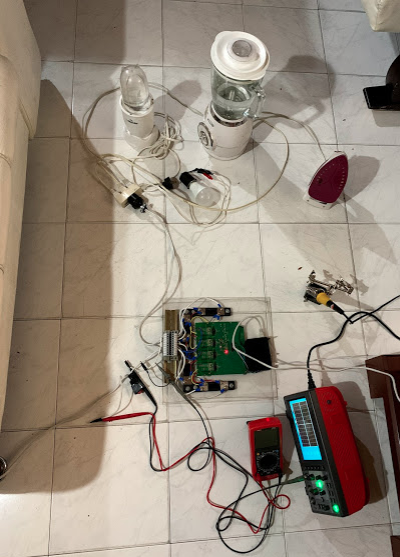
\includegraphics[width = 5cm]{4Resultados/montaje-1.png}
      \caption{ Montaje de la primera prueba } 
      \label{fig:montaje1}
 \end{center}
\end{figure}
  
\section{Segunda Prueba}
  
En esta prueba se decidió medir todo el ciclo de lavado de una lavadora, con el fin de obtener datos en distintos escenarios los cuales seria llenado, lavado y centrifugado y tener una medición más estable.

Carga:

\begin{itemize}
  \itemsep0em
  \item Lavadora whirlpool de 9.8 A.
\end{itemize}

Ciclos de lavado:

\begin{itemize}
  \itemsep0em
  \item Heavy
  \item Regular
  \item Super wash
  \item Centrifugado
  \item Rinse
  \item Llenado
\end{itemize}

El análisis se realizó con respecto a los ciclos de lavado y en los todos los ciclos los siguientes datos fueron comunes:

\begin{itemize}
  \itemsep0em
  \item Volatje RMS total con un valor promedio de 121 V en todos los ciclos.
  \item Volatje RMS Fundamental con un valor promedio de 120,97 V en todos los ciclos.
\end{itemize}

\subsection{Análisis en el ciclo heavy}
\begin{figure}[H]
  \hfill
  \subfigure{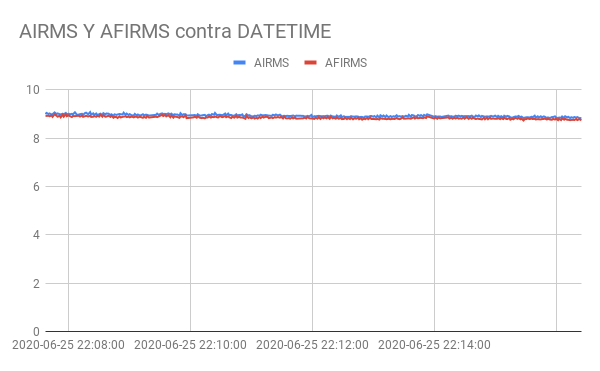
\includegraphics[width=7.5cm]{4Resultados/AIRMS-AFIRMS-Heavy.png}}
  \hfill
  \subfigure{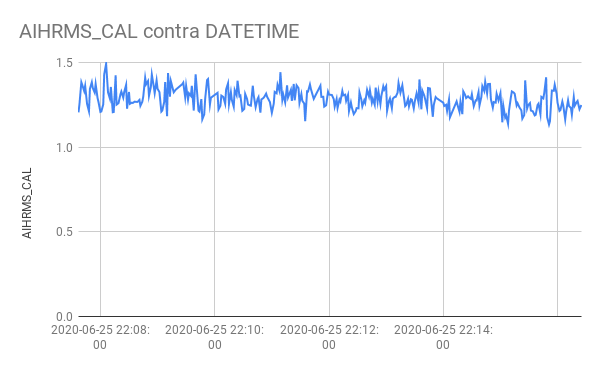
\includegraphics[width=7.5cm]{4Resultados/AIHRMS_CAL-Heavy.png}}
  \hfill
  \caption{AIRMS, AFIRMS Y AIHRMS-CAL VS DATETIME EN EL CICLO HEAVY}
  \end{figure}
\begin{figure}[H]
  \hfill
  \subfigure{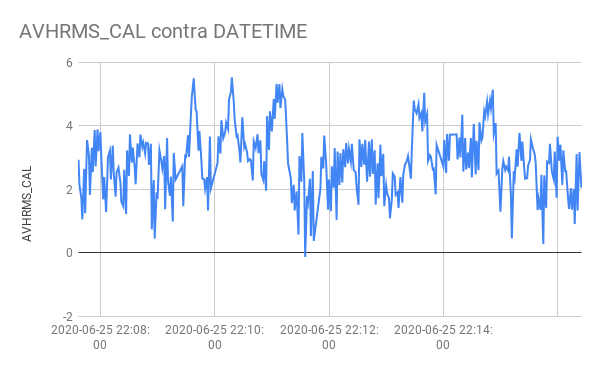
\includegraphics[width=7.5cm]{4Resultados/AVHRMS_CAL-Heavy.png}}
  \hfill
  \subfigure{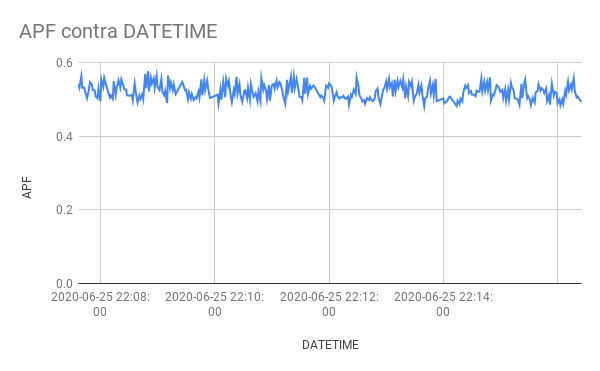
\includegraphics[width=7.5cm]{4Resultados/APF-Heavy.png}}
  \hfill
  \caption{AVHRMS Y APF VS DATETIME EN EL CICLO HEAVY}
  \end{figure}
\begin{figure}[H]
  \hfill
  \subfigure{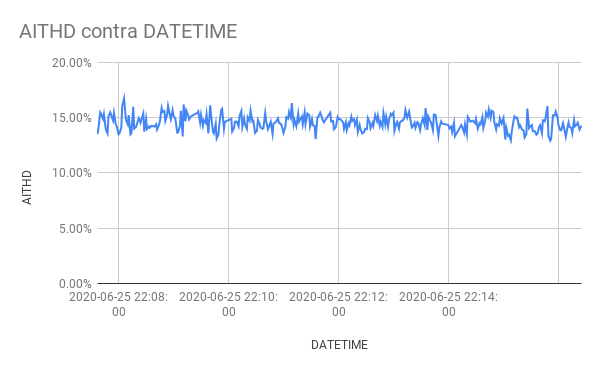
\includegraphics[width=7.5cm]{4Resultados/AITHD-Heavy.png}}
  \hfill
  \subfigure{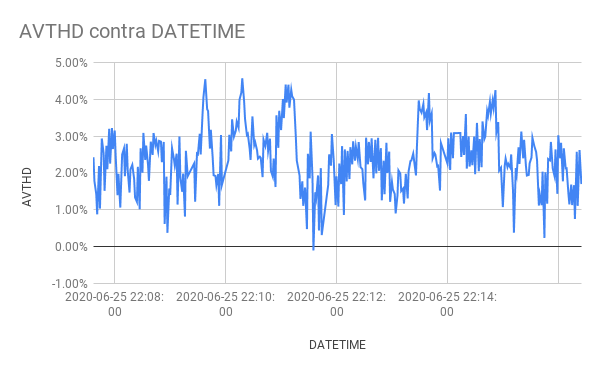
\includegraphics[width=7.5cm]{4Resultados/AVTHD-Heavy.png}}
  \hfill
  \caption{AITHD Y AVTHD VS DATETIME EN EL CICLO HEAVY}
  \end{figure}
\begin{figure}[H]
  \hfill
  \subfigure{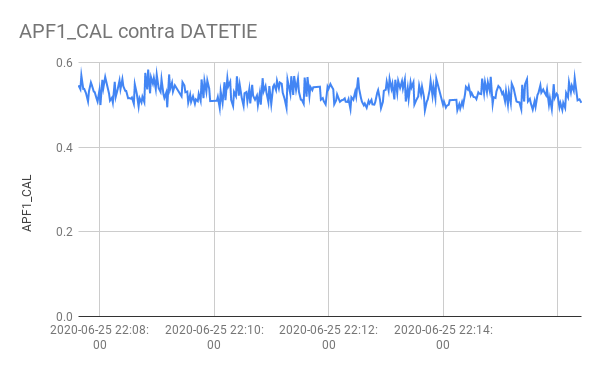
\includegraphics[width=7.5cm]{4Resultados/APF1_CAL-Heavy.png}}
  \hfill
  \subfigure{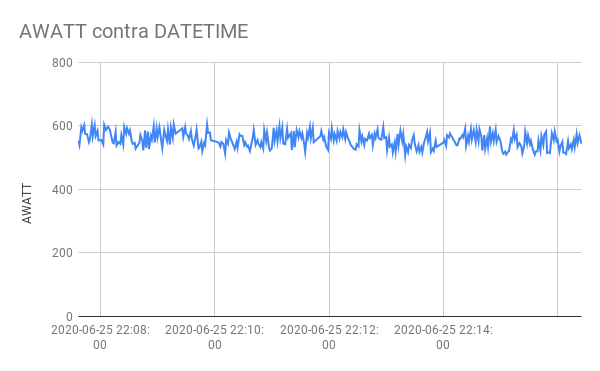
\includegraphics[width=7.5cm]{4Resultados/AWATT-Heavy.png}}
  \hfill
  \caption{APF1-CAL Y AWATT VS DATETIME EN EL CICLO HEAVY}
  \end{figure}
\begin{figure}[H]
  \hfill
  \subfigure{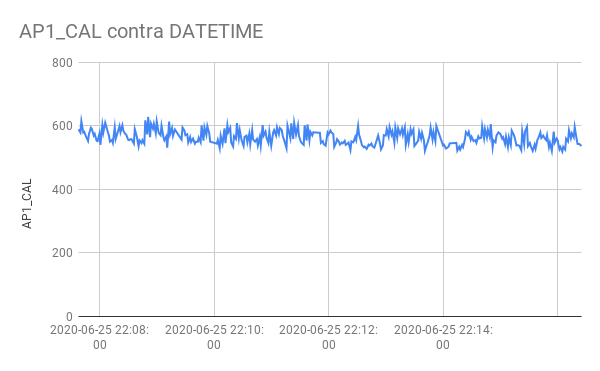
\includegraphics[width=7.5cm]{4Resultados/AP1_CAL-Heavy.png}}
  \hfill
  \subfigure{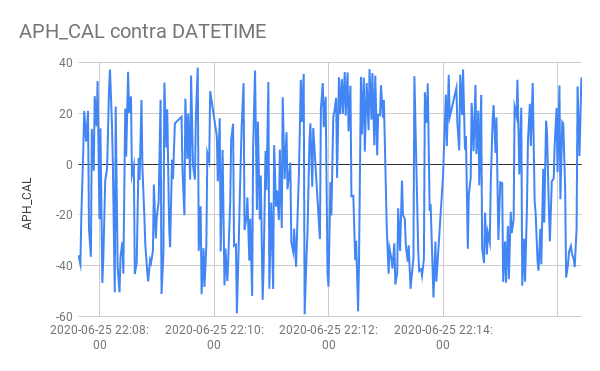
\includegraphics[width=7.5cm]{4Resultados/APH_CAL-Heavy.png}}
  \hfill
  \caption{AP1-CAL Y APH-CAL VS DATETIME EN EL CICLO HEAVY}
  \end{figure}
\begin{figure}[H]
  \hfill
  \subfigure{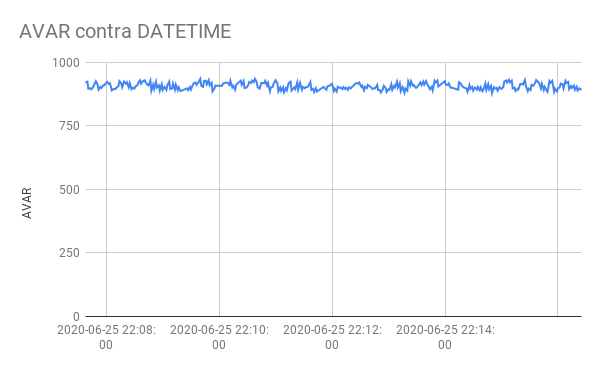
\includegraphics[width=7.5cm]{4Resultados/AVAR-Heavy.png}}
  \hfill
  \subfigure{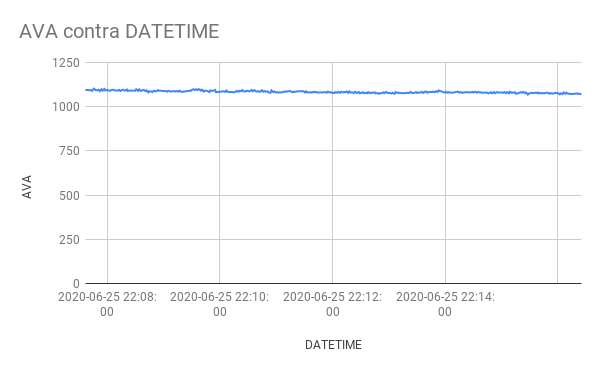
\includegraphics[width=7.5cm]{4Resultados/AVA-Heavy.png}}
  \hfill
  \caption{AVAR Y AVA VS DATETIME EN EL CICLO HEAVY}
  \end{figure}
\begin{figure}[H]
  \hfill
  \subfigure{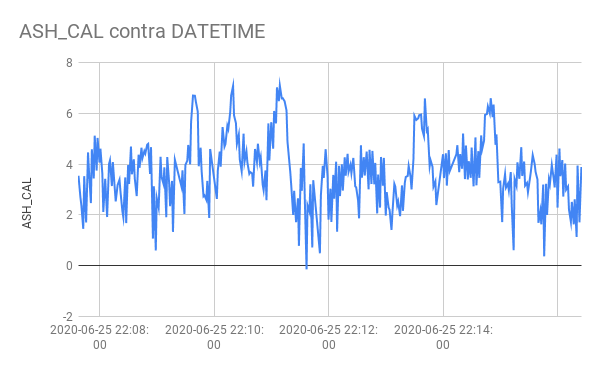
\includegraphics[width=7.5cm]{4Resultados/ASH_CAL-Heavy.png}}
  \hfill
  \subfigure{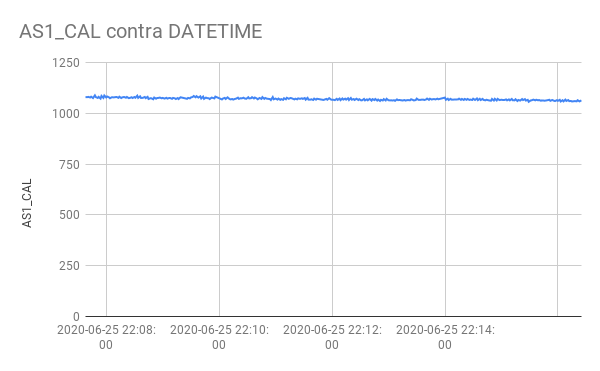
\includegraphics[width=7.5cm]{4Resultados/AS1_CAL-Heavy.png}}
  \hfill
  \caption{ASH-CAL Y AS1-CAL VS DATETIME EN EL CICLO HEAVY}
  \end{figure}
\begin{figure}[H]
  \hfill
  \subfigure{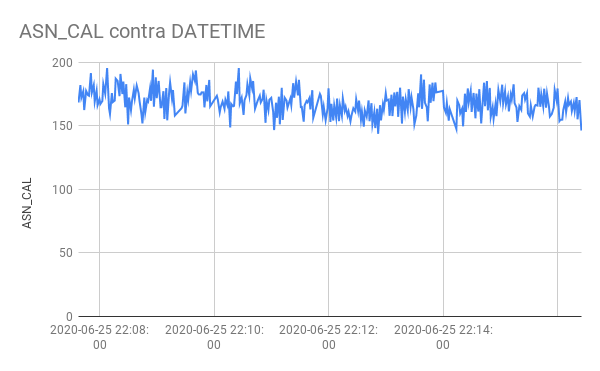
\includegraphics[width=7.5cm]{4Resultados/ASN_CAL-Heavy.png}}
  \hfill
  \subfigure{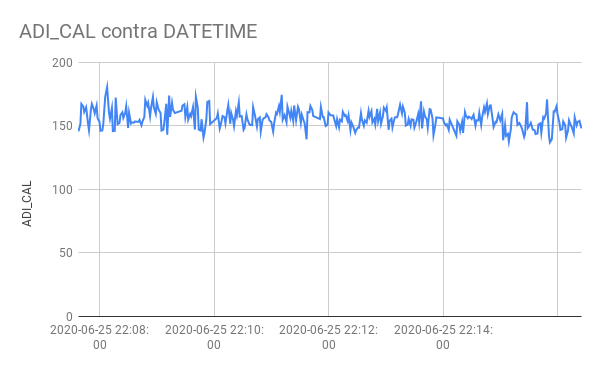
\includegraphics[width=7.5cm]{4Resultados/ADI_CAL-Heavy.png}}
  \hfill
  \caption{ASN-CAL Y ADI-CAL VS DATETIME EN EL CICLO HEAVY}
  \end{figure}
\begin{figure}[H]
  \hfill
  \subfigure{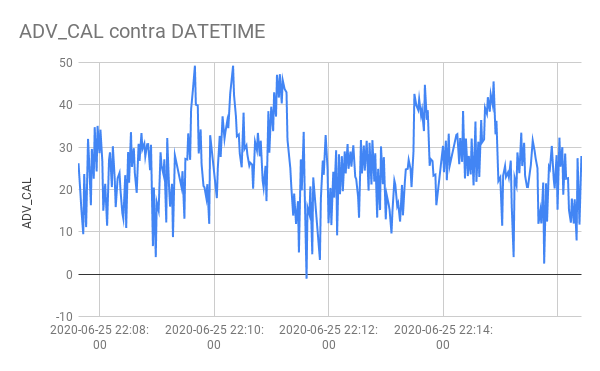
\includegraphics[width=7.5cm]{4Resultados/ADV_CAL-Heavy.png}}
  \hfill
  \subfigure{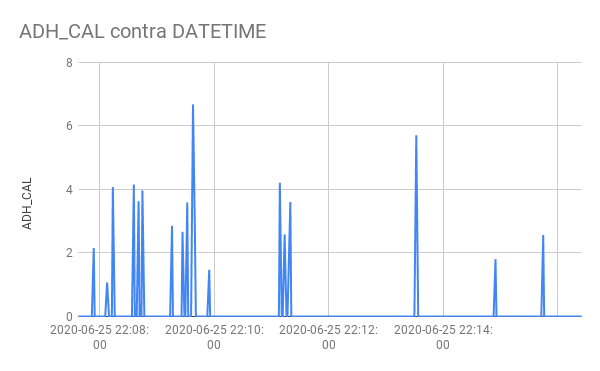
\includegraphics[width=7.5cm]{4Resultados/ADH_CAL-Heavy.png}}
  \hfill
  \caption{ADV-CAL Y ADH-CAL VS DATETIME EN EL CICLO HEAVY}
  \end{figure}
\begin{figure}[H]
  \hfill
  \subfigure{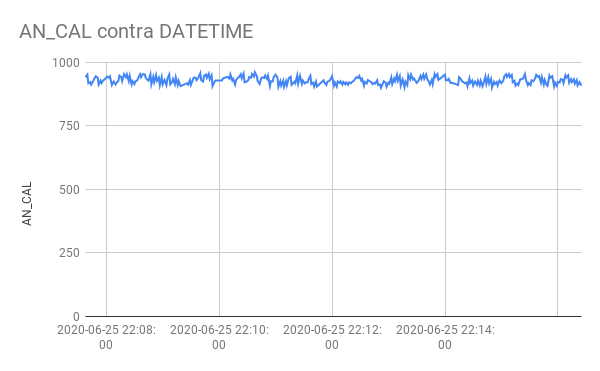
\includegraphics[width=7.5cm]{4Resultados/AN_CAL-Heavy.png}}
  \hfill
  \subfigure{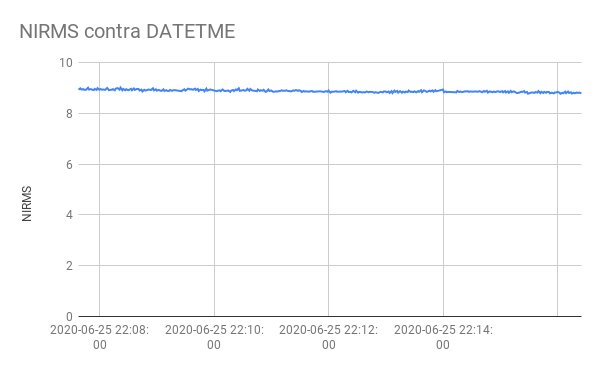
\includegraphics[width=7.5cm]{4Resultados/NIRMS-Heavy.png}}
  \hfill
  \caption{AN-CAL Y NIRMS VS DATETIME EN EL CICLO HEAVY}
  \end{figure}
\begin{figure}[H]
  \hfill
  \subfigure{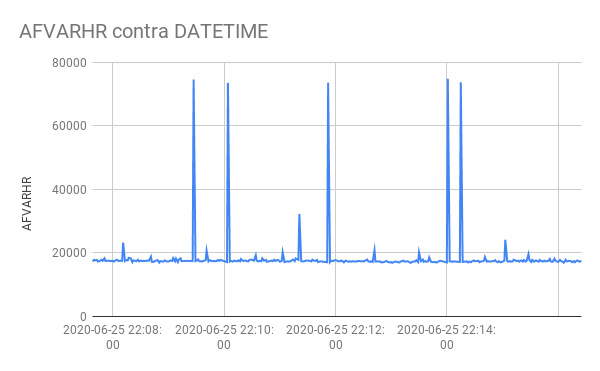
\includegraphics[width=7.5cm]{4Resultados/AFVARHR-Heavy.png}}
  \hfill
  \subfigure{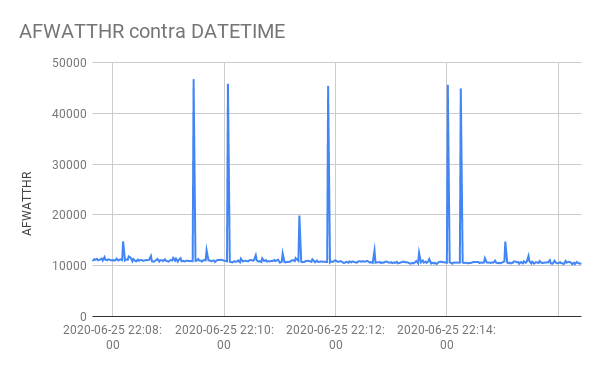
\includegraphics[width=7.5cm]{4Resultados/AFWATTHR-Heavy.png}}
  \hfill
  \caption{AFVARHR Y AFWATTHR VS DATETIME EN EL CICLO HEAVY}
  \end{figure}
\begin{figure}[H]
  \hfill
  \subfigure{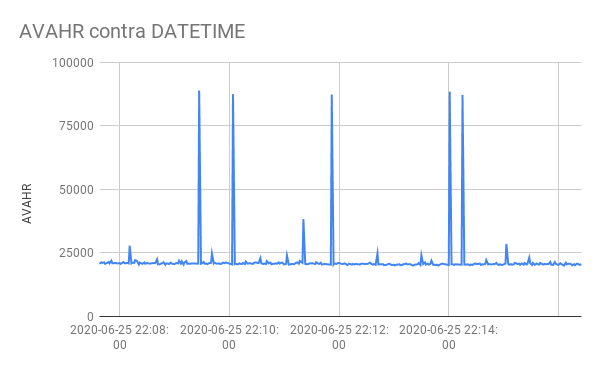
\includegraphics[width=7.5cm]{4Resultados/AVAHR-Heavy.png}}
  \hfill
  \subfigure{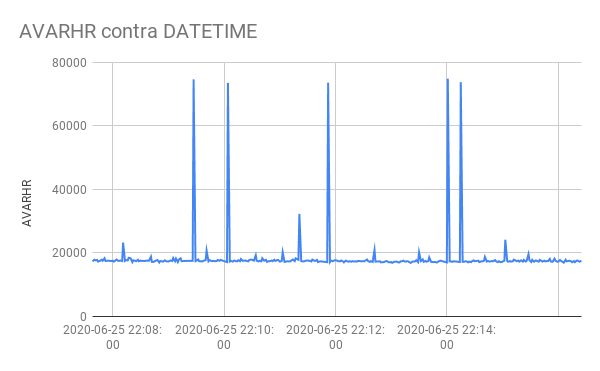
\includegraphics[width=7.5cm]{4Resultados/AVARHR-Heavy.png}}
  \hfill
  \caption{AVAHR Y AVARHR VS DATETIME EN EL CICLO HEAVY}
  \end{figure}
\begin{figure}[H]
  \hfill
  \subfigure{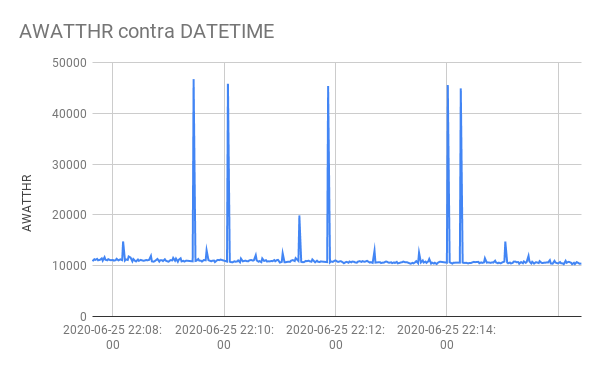
\includegraphics[width=7.5cm]{4Resultados/AWATTHR-Heavy.png}}
  \hfill
  \caption{AWATTHR VS DATETIME EN EL CICLO HEAVY}
  \end{figure}
\subsection{Análisis en el ciclo regular}
\begin{figure}[H]
  \hfill
  \subfigure{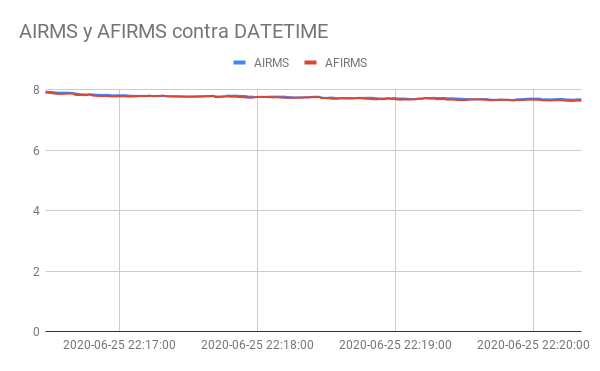
\includegraphics[width=7.5cm]{4Resultados/AIRMS-AFIRMS-Regular.png}}
  \hfill
  \subfigure{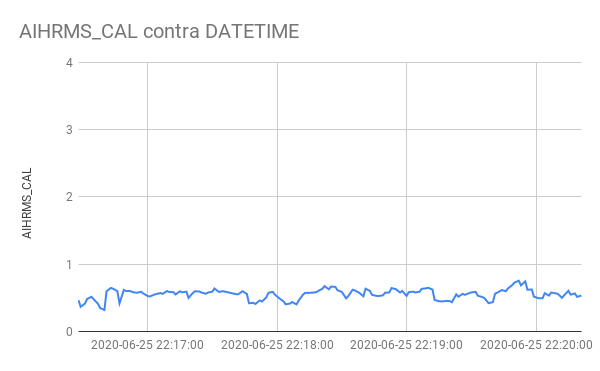
\includegraphics[width=7.5cm]{4Resultados/AIHRMS_CAL-Regular.png}}
  \hfill
  \caption{AIRMS, AFIRMS Y AIHRMS-CAL VS DATETIME EN EL CICLO REGULAR}
  \end{figure}
\begin{figure}[H]
  \hfill
  \subfigure{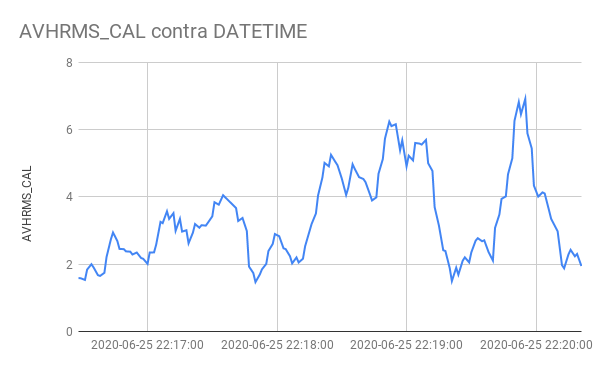
\includegraphics[width=7.5cm]{4Resultados/AVHRMS_CAL-Regular.png}}
  \hfill
  \subfigure{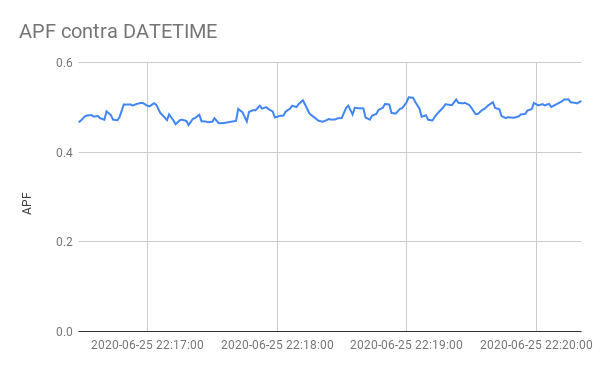
\includegraphics[width=7.5cm]{4Resultados/APF-Regular.png}}
  \hfill
  \caption{AVHRMS Y APF VS DATETIME EN EL CICLO REGULAR}
  \end{figure}
\begin{figure}[H]
  \hfill
  \subfigure{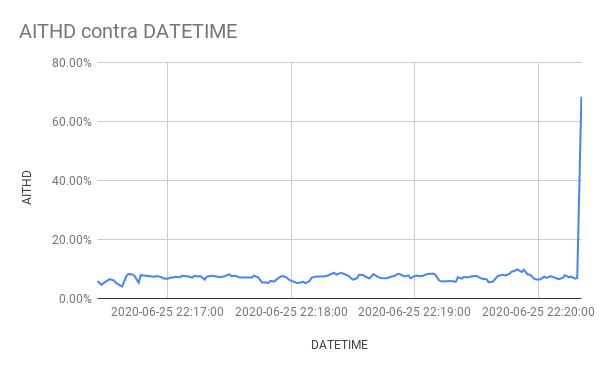
\includegraphics[width=7.5cm]{4Resultados/AITHD-Regular.png}}
  \hfill
  \subfigure{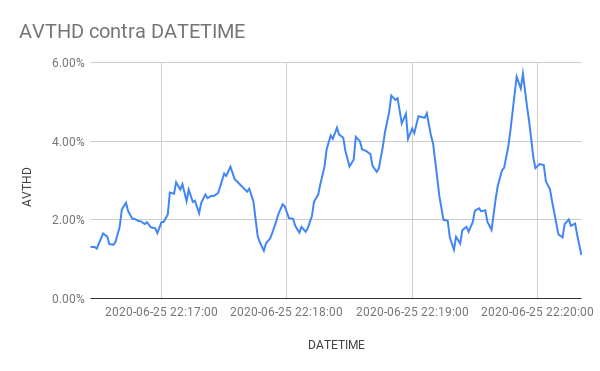
\includegraphics[width=7.5cm]{4Resultados/AVTHD-Regular.png}}
  \hfill
  \caption{AITHD Y AVTHD VS DATETIME EN EL CICLO REGULAR}
  \end{figure}
\begin{figure}[H]
  \hfill
  \subfigure{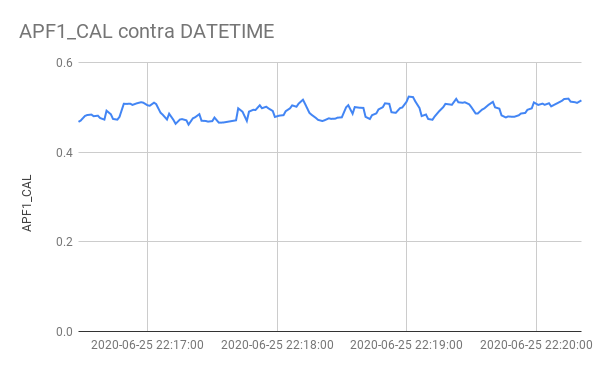
\includegraphics[width=7.5cm]{4Resultados/APF1_CAL-Regular.png}}
  \hfill
  \subfigure{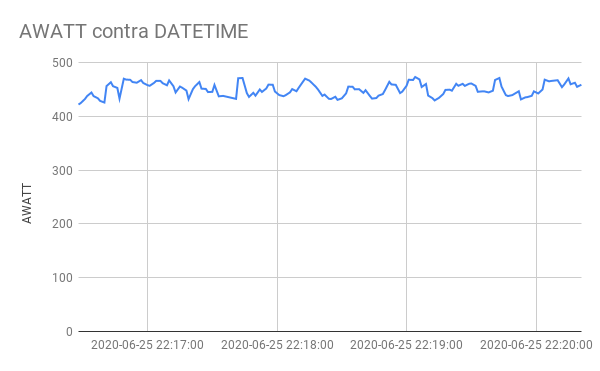
\includegraphics[width=7.5cm]{4Resultados/AWATT-Regular.png}}
  \hfill
  \caption{APF1-CAL Y AWATT VS DATETIME EN EL CICLO REGULAR}
  \end{figure}
\begin{figure}[H]
  \hfill
  \subfigure{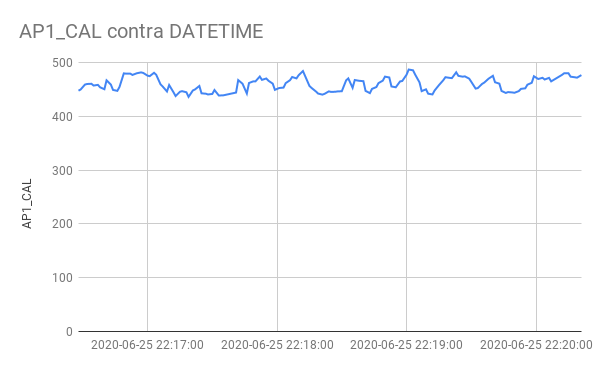
\includegraphics[width=7.5cm]{4Resultados/AP1_CAL-Regular.png}}
  \hfill
  \subfigure{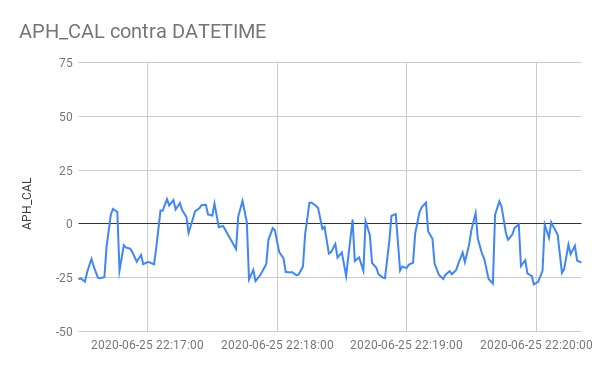
\includegraphics[width=7.5cm]{4Resultados/APH_CAL-Regular.png}}
  \hfill
  \caption{AP1-CAL Y APH-CAL VS DATETIME EN EL CICLO REGULAR}
  \end{figure}
\begin{figure}[H]
  \hfill
  \subfigure{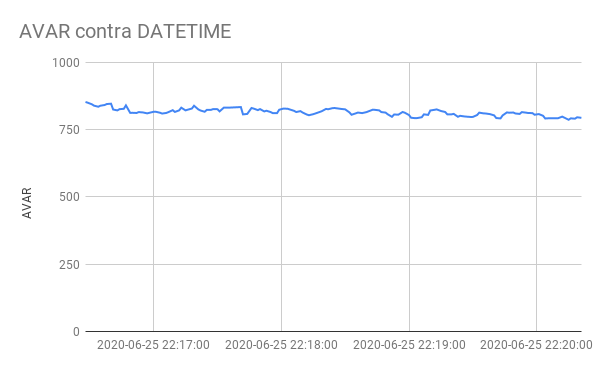
\includegraphics[width=7.5cm]{4Resultados/AVAR-Regular.png}}
  \hfill
  \subfigure{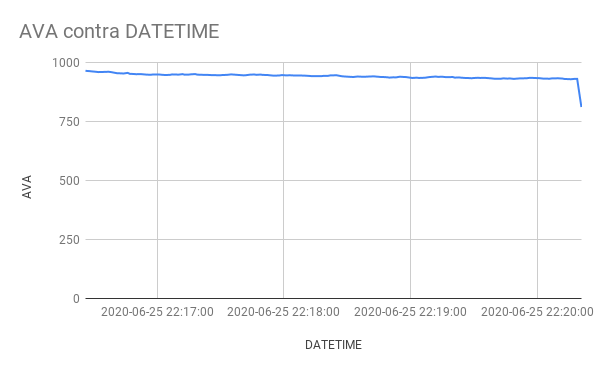
\includegraphics[width=7.5cm]{4Resultados/AVA-Regular.png}}
  \hfill
  \caption{AVAR Y AVA VS DATETIME EN EL CICLO REGULAR}
  \end{figure}
\begin{figure}[H]
  \hfill
  \subfigure{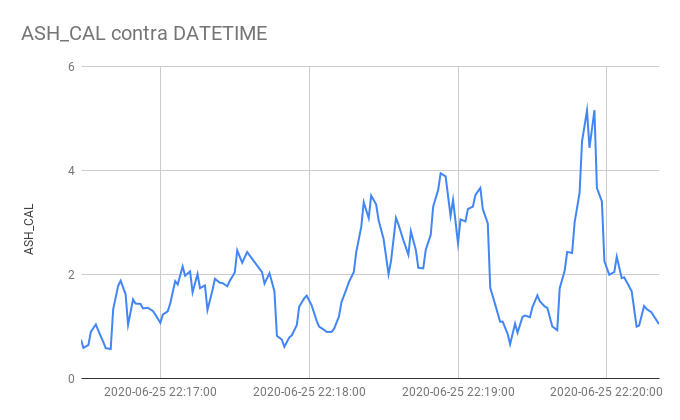
\includegraphics[width=7.5cm]{4Resultados/ASH_CAL-Regular.png}}
  \hfill
  \subfigure{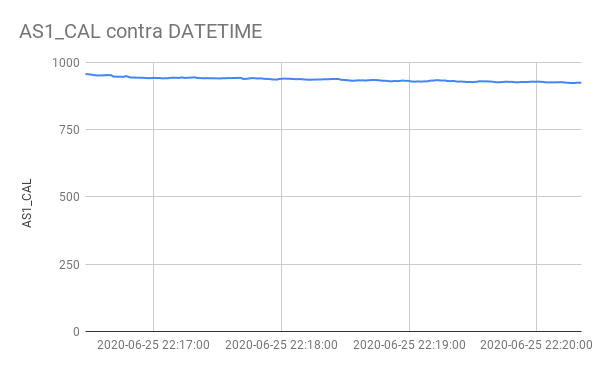
\includegraphics[width=7.5cm]{4Resultados/AS1_CAL-Regular.png}}
  \hfill
  \caption{ASH-CAL Y AS1-CAL VS DATETIME EN EL CICLO REGULAR}
  \end{figure}
\begin{figure}[H]
  \hfill
  \subfigure{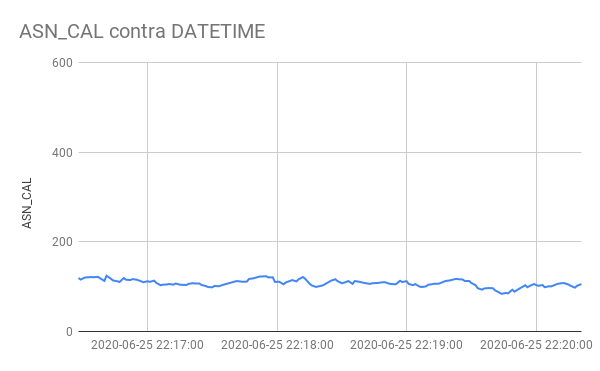
\includegraphics[width=7.5cm]{4Resultados/ASN_CAL-Regular.png}}
  \hfill
  \subfigure{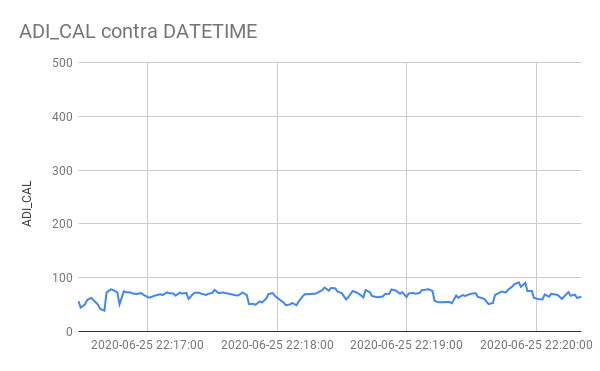
\includegraphics[width=7.5cm]{4Resultados/ADI_CAL-Regular.png}}
  \hfill
  \caption{ASN-CAL Y ADI-CAL VS DATETIME EN EL CICLO REGULAR}
  \end{figure}
\begin{figure}[H]
  \hfill
  \subfigure{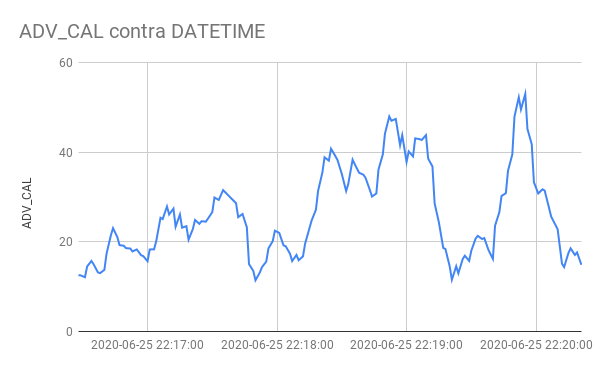
\includegraphics[width=7.5cm]{4Resultados/ADV_CAL-Regular.png}}
  \hfill
  \subfigure{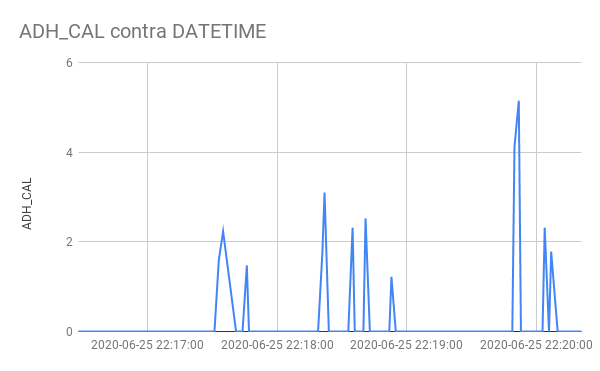
\includegraphics[width=7.5cm]{4Resultados/ADH_CAL-Regular.png}}
  \hfill
  \caption{ADV-CAL Y ADH-CAL VS DATETIME EN EL CICLO REGULAR}
  \end{figure}
\begin{figure}[H]
  \hfill
  \subfigure{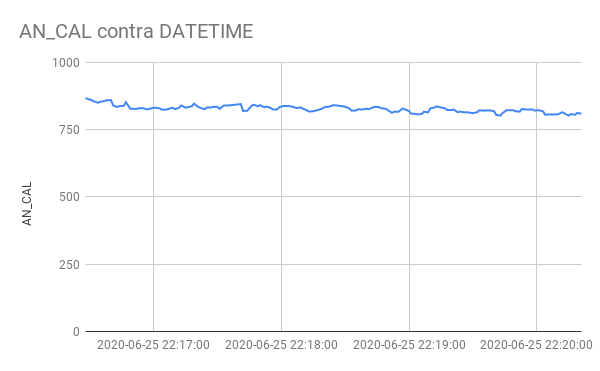
\includegraphics[width=7.5cm]{4Resultados/AN_CAL-Regular.png}}
  \hfill
  \subfigure{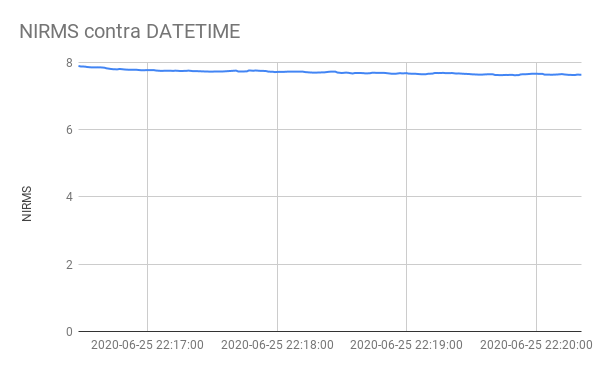
\includegraphics[width=7.5cm]{4Resultados/NIRMS-Regular.png}}
  \hfill
  \caption{AN-CAL Y NIRMS VS DATETIME EN EL CICLO REGULAR}
  \end{figure}
\begin{figure}[H]
  \hfill
  \subfigure{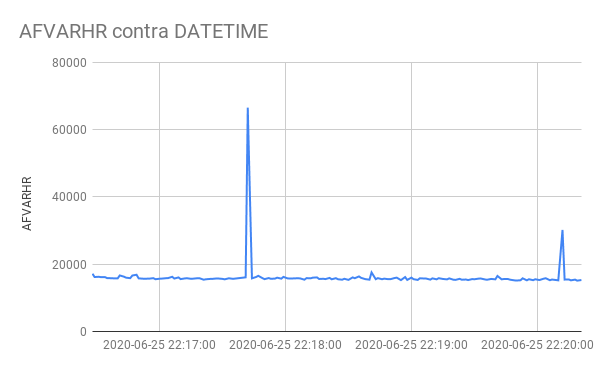
\includegraphics[width=7.5cm]{4Resultados/AFVARHR-Regular.png}}
  \hfill
  \subfigure{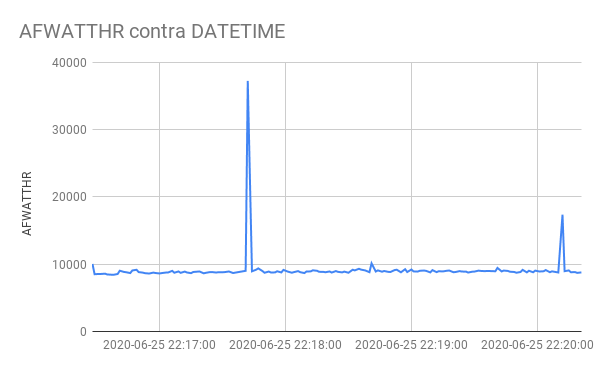
\includegraphics[width=7.5cm]{4Resultados/AFWATTHR-Regular.png}}
  \hfill
  \caption{AFVARHR Y AFWATTHR VS DATETIME EN EL CICLO REGULAR}
  \end{figure}
\begin{figure}[H]
  \hfill
  \subfigure{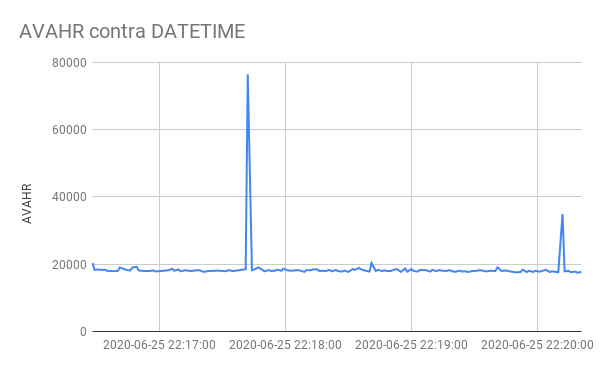
\includegraphics[width=7.5cm]{4Resultados/AVAHR-Regular.png}}
  \hfill
  \subfigure{\includegraphics[width=7.5cm]{4Resultados/AVARHR-Regular.png}}
  \hfill
  \caption{AVAHR Y AVARHR VS DATETIME EN EL CICLO REGULAR}
  \end{figure}
\begin{figure}[H]
  \hfill
  \subfigure{\includegraphics[width=7.5cm]{4Resultados/AWATTHR-Regular.png}}
  \hfill
  \caption{AWATTHR VS DATETIME EN EL CICLO REGULAR}
  \end{figure}
\subsection{Análisis en el ciclo super wash}
\begin{figure}[H]
  \hfill
  \subfigure{\includegraphics[width=7.5cm]{4Resultados/AIRMS-AFIRMS-SuperWash.png}}
  \hfill
  \subfigure{\includegraphics[width=7.5cm]{4Resultados/AIHRMS_CAL-SuperWash.png}}
  \hfill
  \caption{AIRMS, AFIRMS Y AIHRMS-CAL VS DATETIME EN EL CICLO SUPER WASH}
  \end{figure}
\begin{figure}[H]
  \hfill
  \subfigure{\includegraphics[width=7.5cm]{4Resultados/AVHRMS_CAL-SuperWash.png}}
  \hfill
  \subfigure{\includegraphics[width=7.5cm]{4Resultados/APF-SuperWash.png}}
  \hfill
  \caption{AVHRMS Y APF VS DATETIME EN EL CICLO SUPER WASH}
  \end{figure}
\begin{figure}[H]
  \hfill
  \subfigure{\includegraphics[width=7.5cm]{4Resultados/AITHD-SuperWash.png}}
  \hfill
  \subfigure{\includegraphics[width=7.5cm]{4Resultados/AVTHD-SuperWash.png}}
  \hfill
  \caption{AITHD Y AVTHD VS DATETIME EN EL CICLO SUPER WASH}
  \end{figure}
\begin{figure}[H]
  \hfill
  \subfigure{\includegraphics[width=7.5cm]{4Resultados/APF1_CAL-SuperWash.png}}
  \hfill
  \subfigure{\includegraphics[width=7.5cm]{4Resultados/AWATT-SuperWash.png}}
  \hfill
  \caption{APF1-CAL Y AWATT VS DATETIME EN EL CICLO SUPER WASH}
  \end{figure}
\begin{figure}[H]
  \hfill
  \subfigure{\includegraphics[width=7.5cm]{4Resultados/AP1_CAL-SuperWash.png}}
  \hfill
  \subfigure{\includegraphics[width=7.5cm]{4Resultados/APH_CAL-SuperWash.png}}
  \hfill
  \caption{AP1-CAL Y APH-CAL VS DATETIME EN EL CICLO SUPER WASH}
  \end{figure}
\begin{figure}[H]
  \hfill
  \subfigure{\includegraphics[width=7.5cm]{4Resultados/AVAR-SuperWash.png}}
  \hfill
  \subfigure{\includegraphics[width=7.5cm]{4Resultados/AVA-SuperWash.png}}
  \hfill
  \caption{AVAR Y AVA VS DATETIME EN EL CICLO SUPER WASH}
  \end{figure}
\begin{figure}[H]
  \hfill
  \subfigure{\includegraphics[width=7.5cm]{4Resultados/ASH_CAL-SuperWash.png}}
  \hfill
  \subfigure{\includegraphics[width=7.5cm]{4Resultados/AS1_CAL-SuperWash.png}}
  \hfill
  \caption{ASH-CAL Y AS1-CAL VS DATETIME EN EL CICLO SUPER WASH}
  \end{figure}
\begin{figure}[H]
  \hfill
  \subfigure{\includegraphics[width=7.5cm]{4Resultados/ASN_CAL-SuperWash.png}}
  \hfill
  \subfigure{\includegraphics[width=7.5cm]{4Resultados/ADI_CAL-SuperWash.png}}
  \hfill
  \caption{ASN-CAL Y ADI-CAL VS DATETIME EN EL CICLO SUPER WASH}
  \end{figure}
\begin{figure}[H]
  \hfill
  \subfigure{\includegraphics[width=7.5cm]{4Resultados/ADV_CAL-SuperWash.png}}
  \hfill
  \subfigure{\includegraphics[width=7.5cm]{4Resultados/ADH_CAL-SuperWash.png}}
  \hfill
  \caption{ADV-CAL Y ADH-CAL VS DATETIME EN EL CICLO SUPER WASH}
  \end{figure}
\begin{figure}[H]
  \hfill
  \subfigure{\includegraphics[width=7.5cm]{4Resultados/AN_CAL-SuperWash.png}}
  \hfill
  \subfigure{\includegraphics[width=7.5cm]{4Resultados/NIRMS-SuperWash.png}}
  \hfill
  \caption{AN-CAL Y NIRMS VS DATETIME EN EL CICLO SUPER WASH}
  \end{figure}
\begin{figure}[H]
  \hfill
  \subfigure{\includegraphics[width=7.5cm]{4Resultados/AFVARHR-SuperWash.png}}
  \hfill
  \subfigure{\includegraphics[width=7.5cm]{4Resultados/AFWATTHR-SuperWash.png}}
  \hfill
  \caption{AFVARHR Y AFWATTHR VS DATETIME EN EL CICLO SUPER WASH}
  \end{figure}
\begin{figure}[H]
  \hfill
  \subfigure{\includegraphics[width=7.5cm]{4Resultados/AVAHR-SuperWash.png}}
  \hfill
  \subfigure{\includegraphics[width=7.5cm]{4Resultados/AVARHR-SuperWash.png}}
  \hfill
  \caption{AVAHR Y AVARHR VS DATETIME EN EL CICLO SUPER WASH}
  \end{figure}
\begin{figure}[H]
  \hfill
  \subfigure{\includegraphics[width=7.5cm]{4Resultados/AWATTHR-SuperWash.png}}
  \hfill
  \caption{AWATTHR VS DATETIME EN EL CICLO SUPER WASH}
  \end{figure}
\subsection{Análisis en el ciclo centrifugado}
\begin{figure}[H]
  \hfill
  \subfigure{\includegraphics[width=7.5cm]{4Resultados/AIRMS-AFIRMS-Centrifugado.png}}
  \hfill
  \subfigure{\includegraphics[width=7.5cm]{4Resultados/AIHRMS_CAL-Centrifugado.png}}
  \hfill
  \caption{AIRMS, AFIRMS Y AIHRMS-CAL VS DATETIME EN EL CICLO CENTRIFUGADO}
  \end{figure}
\begin{figure}[H]
  \hfill
  \subfigure{\includegraphics[width=7.5cm]{4Resultados/AVHRMS_CAL-Centrifugado.png}}
  \hfill
  \subfigure{\includegraphics[width=7.5cm]{4Resultados/APF-Centrifugado.png}}
  \hfill
  \caption{AVHRMS Y APF VS DATETIME EN EL CICLO CENTRIFUGADO}
  \end{figure}
\begin{figure}[H]
  \hfill
  \subfigure{\includegraphics[width=7.5cm]{4Resultados/AITHD-Centrifugado.png}}
  \hfill
  \subfigure{\includegraphics[width=7.5cm]{4Resultados/AVTHD-Centrifugado.png}}
  \hfill
  \caption{AITHD Y AVTHD VS DATETIME EN EL CICLO CENTRIFUGADO}
  \end{figure}
\begin{figure}[H]
  \hfill
  \subfigure{\includegraphics[width=7.5cm]{4Resultados/APF1_CAL-Centrifugado.png}}
  \hfill
  \subfigure{\includegraphics[width=7.5cm]{4Resultados/AWATT-Centrifugado.png}}
  \hfill
  \caption{APF1-CAL Y AWATT VS DATETIME EN EL CICLO CENTRIFUGADO}
  \end{figure}
\begin{figure}[H]
  \hfill
  \subfigure{\includegraphics[width=7.5cm]{4Resultados/AP1_CAL-Centrifugado.png}}
  \hfill
  \subfigure{\includegraphics[width=7.5cm]{4Resultados/APH_CAL-Centrifugado.png}}
  \hfill
  \caption{AP1-CAL Y APH-CAL VS DATETIME EN EL CICLO CENTRIFUGADO}
  \end{figure}
\begin{figure}[H]
  \hfill
  \subfigure{\includegraphics[width=7.5cm]{4Resultados/AVAR-Centrifugado.png}}
  \hfill
  \subfigure{\includegraphics[width=7.5cm]{4Resultados/AVA-Centrifugado.png}}
  \hfill
  \caption{AVAR Y AVA VS DATETIME EN EL CICLO CENTRIFUGADO}
  \end{figure}
\begin{figure}[H]
  \hfill
  \subfigure{\includegraphics[width=7.5cm]{4Resultados/ASH_CAL-Centrifugado.png}}
  \hfill
  \subfigure{\includegraphics[width=7.5cm]{4Resultados/AS1_CAL-Centrifugado.png}}
  \hfill
  \caption{ASH-CAL Y AS1-CAL VS DATETIME EN EL CICLO CENTRIFUGADO}
  \end{figure}
\begin{figure}[H]
  \hfill
  \subfigure{\includegraphics[width=7.5cm]{4Resultados/ASN_CAL-Centrifugado.png}}
  \hfill
  \subfigure{\includegraphics[width=7.5cm]{4Resultados/ADI_CAL-Centrifugado.png}}
  \hfill
  \caption{ASN-CAL Y ADI-CAL VS DATETIME EN EL CICLO CENTRIFUGADO}
  \end{figure}
\begin{figure}[H]
  \hfill
  \subfigure{\includegraphics[width=7.5cm]{4Resultados/ADV_CAL-Centrifugado.png}}
  \hfill
  \subfigure{\includegraphics[width=7.5cm]{4Resultados/ADH_CAL-Centrifugado.png}}
  \hfill
  \caption{ADV-CAL Y ADH-CAL VS DATETIME EN EL CICLO CENTRIFUGADO}
  \end{figure}
\begin{figure}[H]
  \hfill
  \subfigure{\includegraphics[width=7.5cm]{4Resultados/AN_CAL-Centrifugado.png}}
  \hfill
  \subfigure{\includegraphics[width=7.5cm]{4Resultados/NIRMS-Centrifugado.png}}
  \hfill
  \caption{AN-CAL Y NIRMS VS DATETIME EN EL CICLO CENTRIFUGADO}
  \end{figure}
\begin{figure}[H]
  \hfill
  \subfigure{\includegraphics[width=7.5cm]{4Resultados/AFVARHR-Centrifugado.png}}
  \hfill
  \subfigure{\includegraphics[width=7.5cm]{4Resultados/AFWATTHR-Centrifugado.png}}
  \hfill
  \caption{AFVARHR Y AFWATTHR VS DATETIME EN EL CICLO CENTRIFUGADO}
  \end{figure}
\begin{figure}[H]
  \hfill
  \subfigure{\includegraphics[width=7.5cm]{4Resultados/AVAHR-Centrifugado.png}}
  \hfill
  \subfigure{\includegraphics[width=7.5cm]{4Resultados/AVARHR-Centrifugado.png}}
  \hfill
  \caption{AVAHR Y AVARHR VS DATETIME EN EL CICLO CENTRIFUGADO}
  \end{figure}
\begin{figure}[H]
  \hfill
  \subfigure{\includegraphics[width=7.5cm]{4Resultados/AWATTHR-Centrifugado.png}}
  \hfill
  \caption{AWATTHR VS DATETIME EN EL CICLO CENTRIFUGADO}
  \end{figure}
\subsection{Análisis en el ciclo rinse}
\begin{figure}[H]
  \hfill
  \subfigure{\includegraphics[width=7.5cm]{4Resultados/AIRMS-AFIRMS-Rinse.png}}
  \hfill
  \subfigure{\includegraphics[width=7.5cm]{4Resultados/AIHRMS_CAL-Rinse.png}}
  \hfill
  \caption{AIRMS, AFIRMS Y AIHRMS-CAL VS DATETIME EN EL CICLO RINSE}
  \end{figure}
\begin{figure}[H]
  \hfill
  \subfigure{\includegraphics[width=7.5cm]{4Resultados/AVHRMS_CAL-Rinse.png}}
  \hfill
  \subfigure{\includegraphics[width=7.5cm]{4Resultados/APF-Rinse.png}}
  \hfill
  \caption{AVHRMS Y APF VS DATETIME EN EL CICLO RINSE}
  \end{figure}
\begin{figure}[H]
  \hfill
  \subfigure{\includegraphics[width=7.5cm]{4Resultados/AITHD-Rinse.png}}
  \hfill
  \subfigure{\includegraphics[width=7.5cm]{4Resultados/AVTHD-Rinse.png}}
  \hfill
  \caption{AITHD Y AVTHD VS DATETIME EN EL CICLO RINSE}
  \end{figure}
\begin{figure}[H]
  \hfill
  \subfigure{\includegraphics[width=7.5cm]{4Resultados/APF1_CAL-Rinse.png}}
  \hfill
  \subfigure{\includegraphics[width=7.5cm]{4Resultados/AWATT-Rinse.png}}
  \hfill
  \caption{APF1-CAL Y AWATT VS DATETIME EN EL CICLO RINSE}
  \end{figure}
\begin{figure}[H]
  \hfill
  \subfigure{\includegraphics[width=7.5cm]{4Resultados/AP1_CAL-Rinse.png}}
  \hfill
  \subfigure{\includegraphics[width=7.5cm]{4Resultados/APH_CAL-Rinse.png}}
  \hfill
  \caption{AP1-CAL Y APH-CAL VS DATETIME EN EL CICLO RINSE}
  \end{figure}
\begin{figure}[H]
  \hfill
  \subfigure{\includegraphics[width=7.5cm]{4Resultados/AVAR-Rinse.png}}
  \hfill
  \subfigure{\includegraphics[width=7.5cm]{4Resultados/AVA-Rinse.png}}
  \hfill
  \caption{AVAR Y AVA VS DATETIME EN EL CICLO RINSE}
  \end{figure}
\begin{figure}[H]
  \hfill
  \subfigure{\includegraphics[width=7.5cm]{4Resultados/ASH_CAL-Rinse.png}}
  \hfill
  \subfigure{\includegraphics[width=7.5cm]{4Resultados/AS1_CAL-Rinse.png}}
  \hfill
  \caption{ASH-CAL Y AS1-CAL VS DATETIME EN EL CICLO RINSE}
  \end{figure}
\begin{figure}[H]
  \hfill
  \subfigure{\includegraphics[width=7.5cm]{4Resultados/ASN_CAL-Rinse.png}}
  \hfill
  \subfigure{\includegraphics[width=7.5cm]{4Resultados/ADI_CAL-Rinse.png}}
  \hfill
  \caption{ASN-CAL Y ADI-CAL VS DATETIME EN EL CICLO RINSE}
  \end{figure}
\begin{figure}[H]
  \hfill
  \subfigure{\includegraphics[width=7.5cm]{4Resultados/ADV_CAL-Rinse.png}}
  \hfill
  \subfigure{\includegraphics[width=7.5cm]{4Resultados/ADH_CAL-Rinse.png}}
  \hfill
  \caption{ADV-CAL Y ADH-CAL VS DATETIME EN EL CICLO RINSE}
  \end{figure}
\begin{figure}[H]
  \hfill
  \subfigure{\includegraphics[width=7.5cm]{4Resultados/AN_CAL-Rinse.png}}
  \hfill
  \subfigure{\includegraphics[width=7.5cm]{4Resultados/NIRMS-Rinse.png}}
  \hfill
  \caption{AN-CAL Y NIRMS VS DATETIME EN EL CICLO RINSE}
  \end{figure}
\begin{figure}[H]
  \hfill
  \subfigure{\includegraphics[width=7.5cm]{4Resultados/AFVARHR-Rinse.png}}
  \hfill
  \subfigure{\includegraphics[width=7.5cm]{4Resultados/AFWATTHR-Rinse.png}}
  \hfill
  \caption{AFVARHR Y AFWATTHR VS DATETIME EN EL CICLO RINSE}
  \end{figure}
\begin{figure}[H]
  \hfill
  \subfigure{\includegraphics[width=7.5cm]{4Resultados/AVAHR-Rinse.png}}
  \hfill
  \subfigure{\includegraphics[width=7.5cm]{4Resultados/AVARHR-Rinse.png}}
  \hfill
  \caption{AVAHR Y AVARHR VS DATETIME EN EL CICLO RINSE}
  \end{figure}
\begin{figure}[H]
  \hfill
  \subfigure{\includegraphics[width=7.5cm]{4Resultados/AWATTHR-Rinse.png}}
  \hfill
  \caption{AWATTHR VS DATETIME EN EL CICLO RINSE}
  \end{figure}
\subsection{Análisis en el ciclo llenado}
\begin{figure}[H]
  \hfill
  \subfigure{\includegraphics[width=7.5cm]{4Resultados/AIRMS-AFIRMS-Llenado.png}}
  \hfill
  \subfigure{\includegraphics[width=7.5cm]{4Resultados/AIHRMS_CAL-Llenado.png}}
  \hfill
  \caption{AIRMS, AFIRMS Y AIHRMS-CAL VS DATETIME EN EL CICLO LLENADO}
  \end{figure}
\begin{figure}[H]
  \hfill
  \subfigure{\includegraphics[width=7.5cm]{4Resultados/AVHRMS_CAL-Llenado.png}}
  \hfill
  \subfigure{\includegraphics[width=7.5cm]{4Resultados/APF-Llenado.png}}
  \hfill
  \caption{AVHRMS Y APF VS DATETIME EN EL CICLO LLENADO}
  \end{figure}
\begin{figure}[H]
  \hfill
  \subfigure{\includegraphics[width=7.5cm]{4Resultados/AITHD-Llenado.png}}
  \hfill
  \subfigure{\includegraphics[width=7.5cm]{4Resultados/AVTHD-Llenado.png}}
  \hfill
  \caption{AITHD Y AVTHD VS DATETIME EN EL CICLO LLENADO}
  \end{figure}
\begin{figure}[H]
  \hfill
  \subfigure{\includegraphics[width=7.5cm]{4Resultados/APF1_CAL-Llenado.png}}
  \hfill
  \subfigure{\includegraphics[width=7.5cm]{4Resultados/AWATT-Llenado.png}}
  \hfill
  \caption{APF1-CAL Y AWATT VS DATETIME EN EL CICLO LLENADO}
  \end{figure}
\begin{figure}[H]
  \hfill
  \subfigure{\includegraphics[width=7.5cm]{4Resultados/AP1_CAL-Llenado.png}}
  \hfill
  \subfigure{\includegraphics[width=7.5cm]{4Resultados/APH_CAL-Llenado.png}}
  \hfill
  \caption{AP1-CAL Y APH-CAL VS DATETIME EN EL CICLO LLENADO}
  \end{figure}
\begin{figure}[H]
  \hfill
  \subfigure{\includegraphics[width=7.5cm]{4Resultados/AVAR-Llenado.png}}
  \hfill
  \subfigure{\includegraphics[width=7.5cm]{4Resultados/AVA-Llenado.png}}
  \hfill
  \caption{AVAR Y AVA VS DATETIME EN EL CICLO LLENADO}
  \end{figure}
\begin{figure}[H]
  \hfill
  \subfigure{\includegraphics[width=7.5cm]{4Resultados/ASH_CAL-Llenado.png}}
  \hfill
  \subfigure{\includegraphics[width=7.5cm]{4Resultados/AS1_CAL-Llenado.png}}
  \hfill
  \caption{ASH-CAL Y AS1-CAL VS DATETIME EN EL CICLO LLENADO}
  \end{figure}
\begin{figure}[H]
  \hfill
  \subfigure{\includegraphics[width=7.5cm]{4Resultados/ASN_CAL-Llenado.png}}
  \hfill
  \subfigure{\includegraphics[width=7.5cm]{4Resultados/ADI_CAL-Llenado.png}}
  \hfill
  \caption{ASN-CAL Y ADI-CAL VS DATETIME EN EL CICLO LLENADO}
  \end{figure}
\begin{figure}[H]
  \hfill
  \subfigure{\includegraphics[width=7.5cm]{4Resultados/ADV_CAL-Llenado.png}}
  \hfill
  \subfigure{\includegraphics[width=7.5cm]{4Resultados/ADH_CAL-Llenado.png}}
  \hfill
  \caption{ADV-CAL Y ADH-CAL VS DATETIME EN EL CICLO LLENADO}
  \end{figure}
\begin{figure}[H]
  \hfill
  \subfigure{\includegraphics[width=7.5cm]{4Resultados/AN_CAL-Llenado.png}}
  \hfill
  \subfigure{\includegraphics[width=7.5cm]{4Resultados/NIRMS-Llenado.png}}
  \hfill
  \caption{AN-CAL Y NIRMS VS DATETIME EN EL CICLO LLENADO}
  \end{figure}
\begin{figure}[H]
  \hfill
  \subfigure{\includegraphics[width=7.5cm]{4Resultados/AFVARHR-Llenado.png}}
  \hfill
  \subfigure{\includegraphics[width=7.5cm]{4Resultados/AFWATTHR-Llenado.png}}
  \hfill
  \caption{AFVARHR Y AFWATTHR VS DATETIME EN EL CICLO LLENADO}
  \end{figure}
\begin{figure}[H]
  \hfill
  \subfigure{\includegraphics[width=7.5cm]{4Resultados/AVAHR-Llenado.png}}
  \hfill
  \subfigure{\includegraphics[width=7.5cm]{4Resultados/AVARHR-Llenado.png}}
  \hfill
  \caption{AVAHR Y AVARHR VS DATETIME EN EL CICLO LLENADO}
  \end{figure}
\begin{figure}[H]
  \hfill
  \subfigure{\includegraphics[width=7.5cm]{4Resultados/AWATTHR-Llenado.png}}
  \hfill
  \caption{AWATTHR VS DATETIME EN EL CICLO LLENADO}
  \end{figure}

  Con esta prueba, se obtuvo una caracterización más del medidor, la cuál para un funcionamiento estable y preciso de la tarjeta, es necesario que las cargas consuman como mínimo 1 Amperio, sin embargo, debido a la alta frecuencia con la que el ADE7978 hace la medición, hay ocasiones en que los datos presentan un valor fuera del rango. \\\\
  Completada la prueba monofásica, se procedió a realizar la prueba trifásica desbalanceada con el fin de tener cubierto todos los casos de medición que se planteó en este proyecto.
  \section{Tercer Prueba}

  Para esta prueba se utilizó una red trifásica doméstica y a cada fase se conectó a una carga. las tres cargas son tienen un consumo distinto para así probar y medir el caso trifásico desbalanceado.\\\\
  A continuación se describe las cargas que se usaron:\\
  \begin{itemize}
    \itemsep0em
    \item FASE A - 2 pantallas, 1 cpu, 2 portatiles y una Raspberry.
    \item FASE B - Caminadora eléctrica.
    \item FASE C - Lavadora samsung.
  \end{itemize}
  \begin{figure}[H]
    \hfill
    \subfigure{\includegraphics[width=7.5cm]{4Resultados/lavadora.jpeg}}
    \hfill
    \subfigure{\includegraphics[width=7.5cm]{4Resultados/caminadora.jpeg}}
    \hfill
    \caption{LAVADORA Y CAMINADORA USADAS EN LA PRUEBA}
    \end{figure}
    \begin{figure}[H]
      \begin{center}
          \includegraphics[width = 7.5cm]{4Resultados/cargas.jpeg}
          \caption{ CARGA DE LA FASE A} 
          \label{fig:cargaA}
     \end{center}
    \end{figure}
    \subsection{Resultados de la prueba}
    \begin{figure}[H]
      \hfill
      \subfigure{\includegraphics[width=7.5cm]{4Resultados/corriente-rms.png}}
      \hfill
      \subfigure{\includegraphics[width=7.5cm]{4Resultados/corriente-fundamental.png}}
      \hfill
      \caption{CORRIENTE RMS Y CORRIENTE FUNDAMENTAL}
      \end{figure}

      Las variaciones que se ven en la señal CIRMS es debido a los distintos ciclos que tiene la lavadora mientras realizaba su ciclo de lavado. \\
      La caminadora se le hizo una variación en la velocidad por lo cual se ve una subida en la gráfica de corriente BIRMS.\\
      La carga en la fase A no tuvo ninguna variación durante la medición por lo cual la señal AIRMS es estable.\\
    \begin{figure}[H]
      \hfill
      \subfigure{\includegraphics[width=7.5cm]{4Resultados/corriente-armonica.png}}
      \hfill
      \subfigure{\includegraphics[width=7.5cm]{4Resultados/THDI.png}}
      \hfill
      \caption{CORRIENTE ARMÓNICA Y DISTORSIÓN ARMÓNICA DE CORRIENTE}
      \label{fig:corriente-armonica}
      \end{figure}
      En la gráfica \ref{fig:Voltaje-armonico}, se ve las distorsiones en corriente que presentan las cargas que en los medidores actuales no tienen en cuenta, sin embargo este medidor lo analiza al momento de medir.
    \begin{figure}[H]
      \hfill
      \subfigure{\includegraphics[width=7.5cm]{4Resultados/voltaje-rms.png}}
      \hfill
      \subfigure{\includegraphics[width=7.5cm]{4Resultados/voltaje-fundamental.png}}
      \hfill
      \caption{VOLTAJE RMS Y VOLTAJE FUNDAMENTAL}
      \end{figure}
    \begin{figure}[H]
      \hfill
      \subfigure{\includegraphics[width=7.5cm]{4Resultados/voltaje-armonico.png}}
      \hfill
      \subfigure{\includegraphics[width=7.5cm]{4Resultados/THDV.png}}
      \hfill
      \caption{VOLTAJE ARMÓNICA Y DISTORSIÓN ARMÓNICA DE VOLTAJE}
      \label{fig:Voltaje-armonico}
      \end{figure}

      En la gráfica \ref{fig:Voltaje-armonico}, se ve las distorsiones en voltaje que presentan las cargas que en los medidores actuales no tienen en cuenta, sin embargo este medidor lo analiza al momento de medir.
    \begin{figure}[H]
      \hfill
      \subfigure{\includegraphics[width=7.5cm]{4Resultados/factor-potencia-total.png}}
      \hfill
      \subfigure{\includegraphics[width=7.5cm]{4Resultados/factor-potencia-fundamental.png}}
      \hfill
      \caption{FACTOR DE POTENCIA TOTAL Y FACTOR DE POTENCIA FUNDAMENTAL}
      \label{fig:factor-potencia}
      \end{figure}
      En la gráfica \ref{fig:factor-potencia}, se evidencia un error en la medición del factor de potencia ya que hay valores superiores a 1.
    
    \begin{figure}[H]
      \hfill
      \subfigure{\includegraphics[width=7.5cm]{4Resultados/potencia-aparente-total.png}}
      \hfill
      \subfigure{\includegraphics[width=7.5cm]{4Resultados/potencia-aparente-fundamental.png}}
      \hfill
      \caption{POTENCIA APARENTE TOTAL Y POTENCIA APARENTE FUNDAMENTAL}
      \end{figure}
    \begin{figure}[H]
      \hfill
      \subfigure{\includegraphics[width=7.5cm]{4Resultados/potencia-aparente-armonica.png}}
      \hfill
      \subfigure{\includegraphics[width=7.5cm]{4Resultados/angulo-desfase.png}}
      \hfill
      \caption{POTENCIA APARENTE ARMÓNICA Y ÁNGULO DE DESFASE ENTRE FASES}
      \end{figure}

    En la gráfica de los ángulos de desfase, las etiquetas se interpretan de la siguiente manera:
    \begin{itemize}
      \itemsep0em
      \item ANGLE 0 - ángulo de desfase entre la fase A y B.
      \item ANGLE 1 - ángulo de desfase entre la fase B y C.
      \item ANGLE 2 - ángulo de desfase entre la fase C y A.
    \end{itemize}
    \begin{figure}[H]
      \hfill
      \subfigure{\includegraphics[width=7.5cm]{4Resultados/potencia-activa-total.png}}
      \hfill
      \subfigure{\includegraphics[width=7.5cm]{4Resultados/potencia-activa-armonica.png}}
      \hfill
      \caption{POTENCIA ACTIVA TOTAL Y POTENCIA ACTIVA ARMÓNICA}
      \end{figure}
    \begin{figure}[H]
      \hfill
      \subfigure{\includegraphics[width=7.5cm]{4Resultados/current-distortion-var.png}}
      \hfill
      \subfigure{\includegraphics[width=7.5cm]{4Resultados/voltage-distortion-var.png}}
      \hfill
      \caption{DISTORSIÓN DE POTENCIA (VAR) EN CORRIENTE Y VOLTAJE}
      \end{figure}
    \begin{figure}[H]
      \hfill
      \subfigure{\includegraphics[width=7.5cm]{4Resultados/NIRMS.png}}
      \hfill
      \subfigure{\includegraphics[width=7.5cm]{4Resultados/potencia-noactiva-var.png}}
      \hfill
      \caption{CORRIENTE RMS EN NEUTRO Y POTENCIA (VAR) NO ACTIVA}
      \end{figure}

      En las gráficas de potencia, se analiza que el consumo de energía es acorde a la corriente que consume la carga.

  